% ============================================================================
%  EC8203 Applied Big Data Engineering -- Mini Project Report
%  Smart Grid Energy Monitoring & Billing: a Lambda architecture pipeline
%
%  Build:  pdflatex report.tex  (run twice for cross-references)
%     or:  latexmk -pdf report.tex
%  Every figure is drawn in TikZ/pgfplots from measured values, except the
%  report screenshot in figures/.
%
%  Orange "To complete" boxes mark content that depends on components still
%  being built (serving API, dashboards, Prometheus/Grafana alerting). Search
%  for \pending before submission: none may remain.
% ============================================================================
\documentclass[11pt,a4paper]{article}

\usepackage[T1]{fontenc}
\usepackage[utf8]{inputenc}
\usepackage{lmodern}
\usepackage[a4paper,margin=2.2cm,top=2.3cm,bottom=2.3cm]{geometry}
\usepackage{microtype}
% Keep "--" as two hyphens in code: command-line flags must survive copying.
\DisableLigatures[-]{encoding=T1,family=tt*}
\usepackage{graphicx}
\usepackage{booktabs,tabularx,array,multirow,makecell}
\usepackage[table]{xcolor}
\usepackage{tikz}
\usetikzlibrary{positioning,arrows.meta,fit,backgrounds,calc}
\usepackage{pgfplots}
\pgfplotsset{compat=1.17}
\usepgfplotslibrary{groupplots}
\usepackage[shortlabels,inline]{enumitem}
\usepackage{caption}
\usepackage{fancyhdr}
\usepackage{titlesec}
\usepackage{tcolorbox}
\usepackage{float}
\usepackage[hyphens]{url}
\usepackage[hidelinks]{hyperref}
\usepackage[capitalise,noabbrev]{cleveref}

% -- Look -------------------------------------------------------------------
\definecolor{ink}{HTML}{1B2A33}
\definecolor{accent}{HTML}{14556B}
\definecolor{muted}{HTML}{5A6672}
\definecolor{speedc}{HTML}{C2410C}
\definecolor{batchc}{HTML}{0F766E}
\captionsetup{font=small,labelfont={bf,color=accent},margin=4pt}
\titleformat{\section}{\large\bfseries\color{accent}}{\thesection}{0.6em}{}
\titleformat{\subsection}{\normalsize\bfseries\color{ink}}{\thesubsection}{0.6em}{}
\titlespacing*{\section}{0pt}{12pt plus 3pt}{5pt}
\titlespacing*{\subsection}{0pt}{8pt plus 2pt}{3pt}
\setlength{\parindent}{0pt}
\setlength{\parskip}{4.5pt plus 1pt}
\setlist{itemsep=1.5pt,topsep=2pt,parsep=0pt,leftmargin=1.3em}
\renewcommand{\arraystretch}{1.18}
\pagestyle{fancy}
\fancyhf{}
\fancyhead[L]{\small\color{muted}EC8203 Mini Project -- Smart Grid Lambda Pipeline}
\fancyhead[R]{\small\color{muted}\thepage}
\renewcommand{\headrulewidth}{0.3pt}

\newcommand{\code}[1]{\texttt{\detokenize{#1}}}
\newcommand{\sq}{Q}
\newcommand{\nm}{\tiny\ttfamily\bfseries}  % task names in diagrams
% Content that depends on components still being built.
\newcommand{\pending}[1]{%
  \begin{tcolorbox}[colback=orange!7,colframe=orange!75!black,boxrule=0.6pt,arc=2pt,
    left=5pt,right=5pt,top=3pt,bottom=3pt,fontupper=\small]
  \textbf{To complete:} #1
  \end{tcolorbox}}
\newcommand{\fillin}[1]{\colorbox{orange!15}{\small #1}}

\hypersetup{pdftitle={Smart Grid Energy Monitoring and Billing: A Lambda Architecture Pipeline},
  pdfsubject={EC8203 Applied Big Data Engineering -- Mini Project}}

\begin{document}

% ============================================================================
%  Cover
% ============================================================================
\begin{titlepage}
  \thispagestyle{empty}
  \vspace*{1.2cm}
  {\color{muted}\large EC8203 Applied Big Data Engineering\\[2pt] Mini Project Report}\\[1.6cm]
  {\color{accent}\rule{\linewidth}{1.2pt}}\\[0.5cm]
  {\Huge\bfseries\color{ink} Smart Grid Energy Monitoring\\[4pt] and Billing}\\[0.4cm]
  {\LARGE\color{accent} A Lambda Architecture Pipeline}\\[0.3cm]
  {\color{accent}\rule{\linewidth}{1.2pt}}\\[0.8cm]
  {\large Use Case 3 \,$\cdot$\, Kafka, Spark Structured Streaming, Airflow,\\[2pt]
   Parquet on S3-compatible storage, PostgreSQL}\\[2.2cm]

  \begin{tabular}{@{}ll@{}}
    \toprule
    \textbf{Group member} & \textbf{Registration number} \\
    \midrule
    Ravindu \fillin{full name} & \fillin{reg.\ no.} \\
    Amami \fillin{full name}   & \fillin{reg.\ no.} \\
    Oshani \fillin{full name}  & \fillin{reg.\ no.} \\
    \bottomrule
  \end{tabular}\\[1.6cm]

  \begin{tabular}{@{}ll@{}}
    Repository & \url{https://github.com/Raviyaa27/smartgrid-lambda-pipeline} \\
    Simulated clock & 1 simulated day = 300 real seconds (288$\times$), from 2026-01-01 \\
    Date & \fillin{submission date}
  \end{tabular}
  \vfill
  {\small\color{muted} All figures in this report were measured on the running system unless
  stated otherwise. Domain quantities (dates, windows, lag) are in simulated time; machine
  quantities (run times, latency) are in real time, and each figure says which.}
\end{titlepage}

% ============================================================================
\section{Use case and requirements}
\label{sec:usecase}
% ============================================================================

We chose \textbf{Use Case 3, Smart Grid Energy Monitoring \& Billing}. A utility
wants real-time visibility of grid load and solar contribution from smart meters,
reconciled daily against tariff and billing data that arrives once a day. The
business question is:

\begin{quote}\itshape
What is the current grid load and renewable contribution by zone, and what will
each household's bill look like once daily tariff data is applied to their
consumption?
\end{quote}

\textbf{This is two questions with incompatible service requirements}, and
separating them is the basis of every decision that follows (\cref{tab:q1q2}).
\sq1 is operational: a control room wants a number that is fresh and
approximately right. \sq2 is financial: a bill is regulated, disputable and
must be reproducible years later.

\begin{table}[H]
\centering\small
\caption{The business question decomposed. The two halves differ on every axis that matters for architecture.}
\label{tab:q1q2}
\begin{tabularx}{\linewidth}{@{}l>{\raggedright\arraybackslash}X>{\raggedright\arraybackslash}X@{}}
\toprule
 & \textbf{\sq1 -- Grid operations} & \textbf{\sq2 -- Billing} \\
\midrule
Question & Current load and renewable mix by zone & Household charge once the day's tariff is applied \\
Freshness & $\le 60$\,s & T+1 (next simulated morning) \\
Tolerance for error & High: a late reading moves a zone total by a fraction of a percent & Zero: exact to LKR 0.01 and reproducible on demand \\
Retention & Hours to days & Years (dispute and regulatory window) \\
Recomputation & Never needed & Required: backdated tariffs, late meter uploads, subsidy changes \\
Cost of being wrong & A slightly stale dashboard & A wrong charge, a refund, a compliance breach \\
\bottomrule
\end{tabularx}
\end{table}

From this we derived the requirements the system is built and tested against:

\begin{enumerate}[label=\textbf{R\arabic*},leftmargin=2.2em]
  \item Zone load and renewable share visible within 60\,s of a reading, labelled \emph{provisional}.
  \item Bills exact to the cent, reproducible, and never published provisionally.
  \item Any past day can be \emph{restated} (recomputed and reissued) with its original kept for audit.
  \item Late and retransmitted readings are counted once, on the day they were taken.
  \item Reference data that fails quality checks never produces a bill (fail closed).
  \item Every stage is observable: logged, measured, and alerting on missing data, errors and low renewable share.
\end{enumerate}

\subsection{Simulated clock}
\label{sec:clock}

To show several daily cycles, including restatement, in one session, time is
compressed \textbf{288$\times$: one simulated day lasts 300 real seconds}, starting at
2026-01-01. Seven simulated days take 35 real minutes. Each meter reports every 2
real seconds, which is one reading per \textbf{9.6 simulated minutes}. That gives
about 30{,}000 readings per simulated day for our 200 households. 288$\times$ is the
fastest ratio at which settling day $N$ reliably finishes before day $N{+}1$ ends
(\cref{sec:perf}).

Two rules make the clock trustworthy. First, \emph{no component reads the wall clock
to decide what day it is}. Event times, partition keys, window boundaries and
settlement dates all derive from one \code{SimulatedClock}. Second, the clock's
anchor is stored once, in \code{ops.sim_clock}, and read by every process. An early
version anchored each process at its own start time. Two sources started 30 real
seconds apart then disagreed by 2.4 simulated hours about the date, which would have
broken the join between the two sources at every midnight.

% ============================================================================
\section{Architecture decision: Lambda, not Kappa}
\label{sec:decision}
% ============================================================================

Lambda~\cite{marz2015} runs a batch layer that recomputes from an immutable master
dataset alongside a speed layer that covers the batch layer's latency. Kappa~\cite{kreps2014}
keeps only the stream, and is the right default for most streaming systems: one engine,
one code path, and reprocessing by replaying the log. The burden of proof is on
choosing Lambda.
We compared the two on the four axes the brief names, sized at production scale
for a utility of this kind. That scale is $10^6$ meters $\times$ 1 reading/minute
$=1.44\times10^9$ events/day, about 288\,GB/day raw, and about 736\,TB over a
7-year dispute and retention window.

\begin{table}[H]
\centering\small
\caption{Lambda versus Kappa on the axes that decide this use case.}
\label{tab:axes}
\begin{tabularx}{\linewidth}{@{}l>{\raggedright\arraybackslash}X>{\raggedright\arraybackslash}X@{}}
\toprule
\textbf{Axis} & \textbf{Kappa (single streaming path)} & \textbf{Lambda (speed + batch)} \\
\midrule
Latency & Meets \sq1 and \sq2 from one stream. \emph{Kappa's strongest axis.} & Speed layer meets \sq1; batch layer meets \sq2. \\
Replay & Restating one day needs the log retained for years, or an external archive read by a separate job, which is Lambda under another name. & Re-run one date-parameterised job over one immutable Parquet partition. Targeted and bounded. \\
Cost & $\approx$736\,TB on broker disk, $\times$3 replication $\approx$ \textbf{2.2\,PB of hot storage}, for a handful of restatements per year. & Parquet compresses this data 8--10$\times$: $\approx$\textbf{75\,TB of cold object storage}. Kafka keeps only a 7-day recovery window. \\
Consistency & Achievable, but the serving store is mutated continuously; proving a March bill at a November audit means reasoning about past stream state. & The batch layer is the declared system of record: deterministic output from immutable input. Reproducing a bill is re-running one job. \\
\bottomrule
\end{tabularx}
\end{table}

\textbf{Decision: Lambda.} The argument is not that Lambda is more capable. It is
that this use case contains \emph{two different consistency contracts}, and Lambda
lets each be met on its own terms. The speed layer serves \sq1 from the live stream.
The batch layer serves \sq2 by recomputing each day from an immutable master dataset.
A serving layer merges them under an explicit rule:

\begin{center}\small
\begin{tabular}{@{}ll@{}}
\toprule
\textbf{Figure requested} & \textbf{Served from} \\
\midrule
Zone metrics for a \emph{past} day & \code{batch.*} (settled): the batch view always wins \\
Zone metrics for \emph{today} & \code{speed.*} (provisional), labelled \textsc{provisional} \\
A household bill & \code{batch.*} only; \textbf{no provisional bill is ever published} \\
\bottomrule
\end{tabular}
\end{center}

\subsection{Rejected alternatives}
\begin{itemize}
  \item \textbf{Kappa.} Rejected on replay, cost and audit together. Serving a
  years-long restatement window needs either $\approx$2.2\,PB of replicated broker
  storage for a rarely used capability, or a long-term archive with its own batch
  reader. The second \emph{is} Lambda with the labels removed. \emph{Kappa would win}
  if billing left the scope, or if disputes were limited to a few days, so that Kafka
  retention could cover the whole window.
  \item \textbf{Kappa with the tariff as a compacted topic.} This is the strongest
  Kappa variant: the daily tariff becomes a stream--table join. It solves the join,
  which was never the hard part. Restating March after a backdated tariff still
  means replaying, and so retaining, March's readings.
  \item \textbf{Batch only.} Satisfies \sq2 fully but fails \sq1: a daily job cannot
  meet a 60-second freshness target or raise a low-renewable alert in time.
\end{itemize}

\subsection{Answering Lambda's known weakness}
Kreps' critique of Lambda~\cite{kreps2014} is that the same logic written for two
engines inevitably diverges, and it is correct as stated. We answered it
structurally, not by discipline:
\begin{enumerate*}[label=(\roman*)]
  \item both layers run on \textbf{one engine}, Spark~3.5.9, with the same connector jars;
  \item validation rules are declared \textbf{once, as data} (a \code{FieldSpec} table), and
  a row-by-row validator and a vectorised validator are both thin adapters over it,
  imported by both layers;
  \item a \textbf{fuzz test} over 4{,}800 damaged messages holds the two validators to identical
  verdicts. It found a real defect: an infinite timestamp crashed both validators,
  which in Spark would have become a poison message replayed forever; and
  \item the approximation the speed layer makes is \textbf{measured}, not asserted, by
  reconciling it against every settlement (\cref{sec:results}).
\end{enumerate*}

% ============================================================================
\section{System architecture}
\label{sec:arch}
% ============================================================================

\begin{figure}[H]
\centering
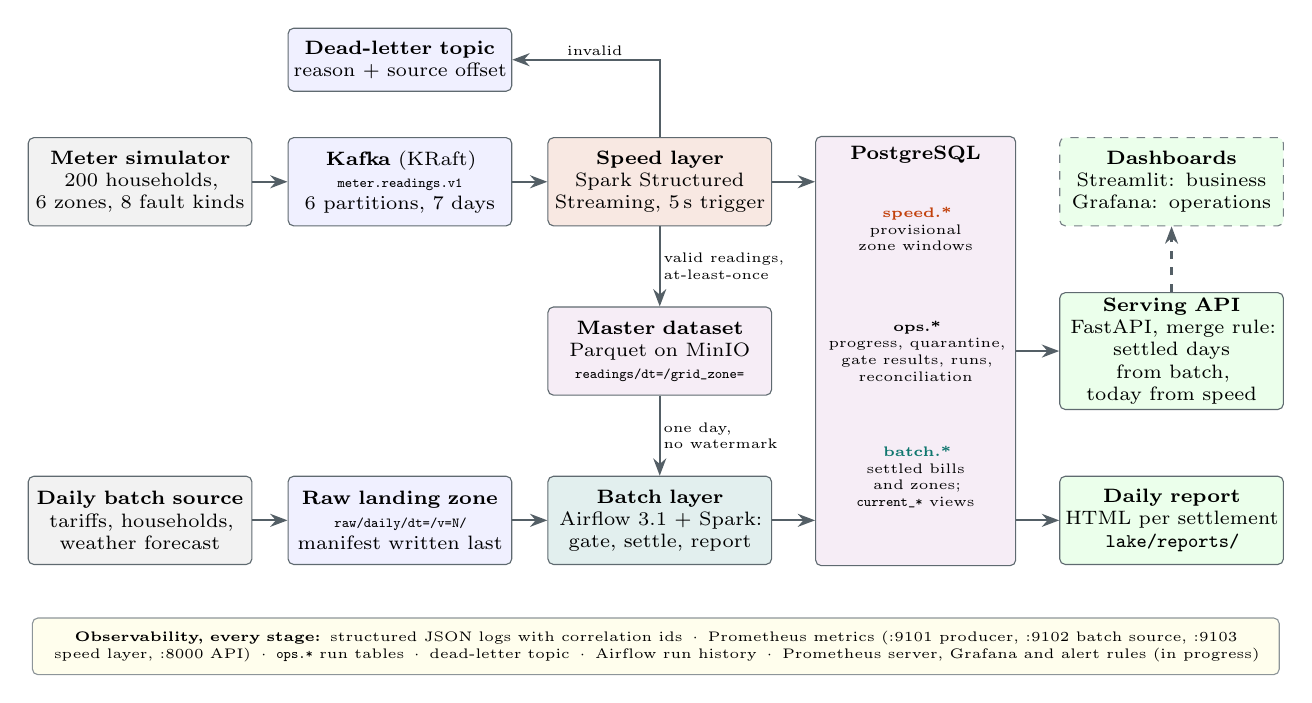
\begin{tikzpicture}[
  font=\scriptsize, >={Stealth[length=2.2mm]},
  box/.style={draw=ink!70, rounded corners=2pt, align=center, minimum height=1.12cm,
              text width=2.7cm, inner sep=2pt},
  src/.style={box, fill=gray!10},
  ing/.style={box, fill=blue!6},
  spd/.style={box, fill=speedc!12},
  bat/.style={box, fill=batchc!12},
  sto/.style={box, fill=violet!7},
  srv/.style={box, fill=green!8},
  wip/.style={dashed, draw=ink!60},
  flow/.style={->, thick, draw=ink!75},
  side/.style={font=\tiny, align=left, inner sep=1pt},
]
% -- speed path (top row)
\node[src] (meter) at (0,4.3) {\textbf{Meter simulator}\\200 households,\\6 zones, 8 fault kinds};
\node[ing] (kafka) at (3.3,4.3) {\textbf{Kafka} (KRaft)\\{\tiny\code{meter.readings.v1}}\\6 partitions, 7 days};
\node[spd] (speed) at (6.6,4.3) {\textbf{Speed layer}\\Spark Structured\\Streaming, 5\,s trigger};
\node[ing, minimum height=0.8cm] (dlq) at (3.3,5.85) {\textbf{Dead-letter topic}\\reason + source offset};
% -- master dataset (middle)
\node[sto] (lake) at (6.6,2.15) {\textbf{Master dataset}\\Parquet on MinIO\\{\tiny\code{readings/dt=/grid_zone=}}};
% -- batch path (bottom row)
\node[src] (daily) at (0,0) {\textbf{Daily batch source}\\tariffs, households,\\weather forecast};
\node[ing] (raw) at (3.3,0) {\textbf{Raw landing zone}\\{\tiny\code{raw/daily/dt=/v=N/}}\\manifest written last};
\node[bat] (batch) at (6.6,0) {\textbf{Batch layer}\\Airflow 3.1 + Spark:\\gate, settle, report};
% -- serving store (tall)
\node[sto, minimum height=5.45cm, text width=2.4cm] (pg) at (9.85,2.15) {};
\node[font=\scriptsize\bfseries, anchor=north] at (pg.north) {PostgreSQL};
\node[font=\tiny, align=center, text width=2.3cm] at ($(pg.center)+(0,1.55)$) {\textbf{\color{speedc}speed.*}\\provisional zone windows};
\node[font=\tiny, align=center, text width=2.3cm] at ($(pg.center)+(0,0)$) {\textbf{ops.*}\\progress, quarantine,\\gate results, runs,\\reconciliation};
\node[font=\tiny, align=center, text width=2.3cm] at ($(pg.center)+(0,-1.6)$) {\textbf{\color{batchc}batch.*}\\settled bills and zones;\\\code{current_*} views};
% -- serving (right column)
\node[srv] (api) at (13.1,2.15) {\textbf{Serving API}\\FastAPI, merge rule:\\settled days from batch,\\today from speed};
\node[srv, wip] (dash) at (13.1,4.3) {\textbf{Dashboards}\\Streamlit: business\\Grafana: operations};
\node[srv] (report) at (13.1,0) {\textbf{Daily report}\\HTML per settlement\\\code{lake/reports/}};
% -- flows
\draw[flow] (meter) -- (kafka);
\draw[flow] (kafka) -- (speed);
\draw[flow] (speed.north) |- node[side, pos=0.72, above] {invalid} (dlq.east);
\draw[flow] (speed) -- node[side, right] {valid readings,\\at-least-once} (lake);
\draw[flow] (lake) -- node[side, right] {one day,\\no watermark} (batch);
\draw[flow] (daily) -- (raw);
\draw[flow] (raw) -- (batch);
\draw[flow] (speed.east) -- (speed.east -| pg.west);
\draw[flow] (batch.east) -- (batch.east -| pg.west);
\draw[flow] (pg.east |- api.west) -- (api.west);
\draw[flow, dashed] (api) -- (dash);
\draw[flow] (pg.east |- report.west) -- (report.west);
% -- observability band
\node[draw=ink!50, fill=yellow!7, rounded corners=2pt, text width=15.6cm, minimum height=0.72cm,
      align=center, font=\tiny] (obs) at (6.55,-1.6)
  {\textbf{Observability, every stage:} structured JSON logs with correlation ids \,$\cdot$\,
   Prometheus metrics (:9101 producer, :9102 batch source, :9103 speed layer, :8000 API) \,$\cdot$\,
   \code{ops.*} run tables \,$\cdot$\, dead-letter topic \,$\cdot$\, Airflow run history
   \,$\cdot$\, Prometheus server, Grafana and alert rules (in progress)};
\end{tikzpicture}
\caption{Architecture. The top row is the speed path (\sq1), the bottom row the batch path (\sq2). They share the
Parquet master dataset, which the speed layer writes and the batch layer recomputes from. PostgreSQL keeps
provisional (\code{speed}) and settled (\code{batch}) figures in separate schemas, so a consumer cannot confuse
them. Every component reads one simulated clock, anchored in \code{ops.sim_clock}. Dashed components are being built.}
\label{fig:arch}
\end{figure}

\textbf{Speed path.} The meter simulator publishes JSON readings to Kafka, keyed by
\code{meter_id} so that each meter's readings stay in order within one partition. A
Spark Structured Streaming job validates every message with the shared validator.
It sends rejects to a dead-letter topic with their reason and source offset. It
appends valid readings to the master dataset, and maintains per-zone, 15-minute
figures in \code{speed.zone_metrics}.

\textbf{Batch path.} Once per simulated day the batch source publishes an immutable,
versioned \emph{drop}: the tariff schedule, each household's tier and subsidy flag,
and a weather forecast per zone. It is complete only when its manifest exists. An
Airflow DAG waits for that drop and for the archive to pass the end of the day. It
then gates the drop and runs a Spark settlement over the whole day. Each settlement
writes a new \emph{run}, which is never overwritten.

\textbf{Storage.} Kafka is transport and short-term recovery (7 days), \emph{not} the
system of record. That is Parquet on MinIO, partitioned by \code{dt} and
\code{grid_zone}. MinIO speaks the S3 API, so moving to AWS changes an endpoint, not
code. PostgreSQL holds only aggregates and bills, in three schemas that encode the
merge rule in the storage layer itself.

% ============================================================================
\section{Technology stack and justification}
\label{sec:stack}
% ============================================================================

Each choice is justified against this use case's constraints rather than general
popularity (\cref{tab:stack}), using the tools' documented guarantees~\cite{kafka,spark,airflow}. One theme runs through them: \emph{the batch layer's
ability to recompute a day exactly} is the requirement most choices serve.

\begin{table}[H]
\centering\small
\caption{Technology stack. Every component runs from one \code{docker compose up}; versions are pinned.}
\label{tab:stack}
\begin{tabularx}{\linewidth}{@{}>{\raggedright\arraybackslash}p{2.05cm}>{\raggedright\arraybackslash}p{2.55cm}>{\raggedright\arraybackslash}X>{\raggedright\arraybackslash}p{2.6cm}@{}}
\toprule
\textbf{Layer} & \textbf{Choice} & \textbf{Why, for this use case} & \textbf{Rejected} \\
\midrule
Ingestion & Kafka 7.6 (KRaft), 6 partitions keyed by meter, 7-day retention & A replayable log. The speed layer restarts from its checkpointed offsets. Per-meter ordering where deduplication needs it. Retention sized to \emph{recovery}, not restatement: the configuration line that encodes the Lambda choice. & RabbitMQ (no replay); Kinesis (no local reproducibility) \\
Stream processing & Spark 3.5 Structured Streaming & Native event-time windows and watermarks for late meter reads; exactly-once effects via checkpoints and idempotent sinks; \textbf{the same engine as the batch layer}, which contains Lambda's drift risk. & Storm (no event time, no batch reuse); Flink (outside the named stack) \\
Batch processing & Spark 3.5 (batch), same image and jars & One artefact, two modes. Settlement re-validates with the same code the speed layer used. & A separate pandas job \\
Orchestration & Airflow 3.1 & Sensors for the late daily file; per-task retries separating transient from fatal errors; the quality gate as a task that fails closed; run history as the settlement audit trail; restatement is re-triggering the DAG for a date. & cron (no dependencies, no history); Dagster (outside the stack) \\
Master dataset & Parquet on MinIO (S3 API) & Columnar and compressed (8--10$\times$); partitioning by date makes ``recompute one day'' read exactly one partition; immutable input makes bills reproducible. & HDFS (a NameNode for no benefit); raw rows in PostgreSQL \\
Serving store & PostgreSQL 16; schemas \code{speed}, \code{batch}, \code{ops} & Serving queries are relational and ad hoc (household $\bowtie$ tariff $\bowtie$ zone). Serving volume is aggregates, orders of magnitude below raw readings. & Cassandra (no ad hoc joins; query-first modelling) \\
Serving \& dashboards & FastAPI; Streamlit (business); Grafana (operations) & One API applies the merge rule so no consumer can bypass it; separate business and operations views for separate audiences. & -- \\
Observability & JSON logs, Prometheus, Grafana & Metrics per stage with a pull model; logs that machines can filter by run, batch or correlation id. & Unstructured logs \\
\bottomrule
\end{tabularx}
\end{table}

\textbf{Versions were chosen, not defaulted.} Airflow 2 reached end of life in April 2026,
so we used Airflow~3.1. Its dependency constraints pin PySpark~4.0.1, while the speed
layer runs 3.5.9. We therefore install PySpark 3.5.9 separately in the Airflow image,
so that both layers run exactly the same engine. Otherwise the ``one engine''
argument above would have been silently false.

% ============================================================================
\section{Implementation}
\label{sec:impl}
% ============================================================================

\subsection{Simulated data sources}
\label{sec:sources}

\textbf{Streaming source.} Each of 200 households has a meter in one of 6 grid zones
and a tariff tier. Consumption follows a daily load curve normalised so a household's
average draw is its true base load. Rooftop solar is zero at night, peaks at noon,
never exceeds rated capacity, and follows each zone's \emph{actual} weather. The daily
drop publishes a \emph{forecast}, so forecast and outcome differ as they do in reality.
Energy is integrated over the simulated interval a reading covers (9.6 minutes).
Integrating over real seconds would undercount by 288$\times$, and a regression test
pins this. The producer is idempotent with \code{acks=all}, and stamps a correlation id
in each payload and Kafka header.

\textbf{Daily batch source.} At 00:30 simulated time it publishes the day's drop as a
new immutable version under \code{raw/daily/dt=D/v=N/}. A drop holds the tariff
schedule, every household's tier and subsidy flag, the weather forecast per zone, and a
manifest. The tariff is \emph{data}, not code. \code{TariffSchedule} carries block rates per tier, fixed charges, the solar
export credit and the subsidy fraction, as decimal strings so no amount passes through
a float. A backdated revision (\code{revise}) or a corrected republish (\code{publish})
becomes version $N{+}1$, beside the original. The manifest is written last, with each
file's SHA-256 and record count, so a half-uploaded drop is never read.

\textbf{Faults are injected on purpose, with ground truth.} A pipeline is only shown
to be robust by feeding it the faults it claims to handle (\cref{tab:faults}). The
stream carries the injected fault in an \code{injected_fault} Kafka header that the
pipeline never reads. Detection can therefore be \emph{measured} against ground truth.

\begin{table}[H]
\centering\small
\caption{Injected faults and the component that handles each.}
\label{tab:faults}
\begin{tabularx}{\linewidth}{@{}>{\raggedright\arraybackslash}p{3.1cm}>{\raggedright\arraybackslash}X>{\raggedright\arraybackslash}p{4.4cm}@{}}
\toprule
\textbf{Fault} & \textbf{Injected as} & \textbf{Handled by} \\
\midrule
\multicolumn{3}{@{}l}{\emph{Streaming source (realistic profile: 2.7\% of messages)}} \\
Content (5 kinds) & missing field, negative value, 60\,kWh spike, malformed JSON, unknown household & Shared validator $\rightarrow$ dead-letter topic with reason \\
Duplicate & The same reading retransmitted & Deduplicated by \code{event_id}: speed layer within watermark; batch layer over the whole day \\
Late & Held back, released after the watermark & Missed by the speed layer (by design), recovered by settlement \\
Backfill & A meter offline for hours, then uploading its backlog & As late: counted on the day it was taken \\
\midrule
\multicolumn{3}{@{}l}{\emph{Daily batch source (drawn per day from a seed)}} \\
Late / missing drop & Arrives after its day ends / never arrives & Airflow sensor waits, then times out and fails the run \\
Source corruption (5) & negative rate, unknown tier, missing or duplicated households, invalid record & Quality gate, validity checks: fails closed \\
Transit corruption & File truncated in transit & Quality gate, integrity: checksum and record count \\
\bottomrule
\end{tabularx}
\end{table}

\subsection{Speed layer}
\label{sec:speed}

Two streaming queries read the same topic, each with its own checkpoint:

\begin{itemize}
  \item \textbf{\code{ingest}} (stateless, \code{foreachBatch}) validates each micro-batch
  with the shared vectorised validator, as a pandas function inside Spark. It appends
  valid readings to the master dataset, partitioned by \code{dt} and \code{grid_zone},
  and sends rejects to the dead-letter topic. It records each micro-batch in \code{ops.*} keyed by
  (simulation, batch id), so a replayed batch after a crash is recorded once.
  \item \textbf{\code{zone_metrics}} (stateful, event time~\cite{kleppmann2017}) applies a
  30-simulated-minute watermark and deduplicates by \code{event_id} within it. It then aggregates 15-minute
  tumbling windows per zone: consumption, solar generation, net energy, average grid
  load, renewable share, readings and meters reporting. Changed windows are
  \emph{upserted} on (zone, window start), so a replay converges rather than double
  counts.
\end{itemize}

\textbf{A design correction found while building.} The obvious design deduplicates
readings before archiving them. In a stream, deduplication must be bounded by a
watermark. A watermark-bounded operator also \emph{discards every reading older than
the watermark}, and those late readings are exactly what the batch layer exists to
recover. The archive therefore keeps every valid reading, written at-least-once, and
deduplication happens where it is safe: in the real-time view, and over the whole day
in settlement (recorded as an ADR amendment).

\subsection{Batch layer}
\label{sec:batch}

\begin{figure}[H]
\centering
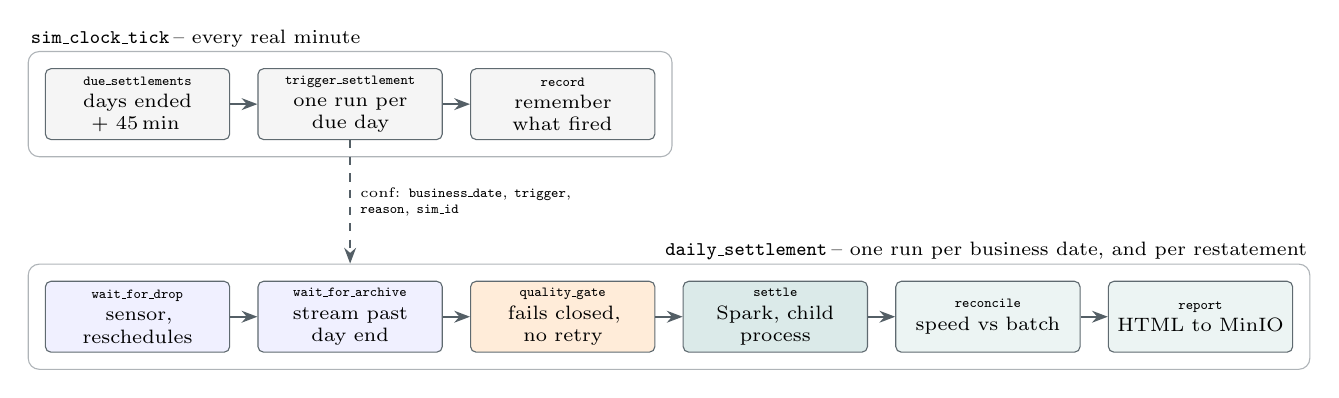
\begin{tikzpicture}[font=\scriptsize, >={Stealth[length=2mm]},
  t/.style={draw=ink!70, rounded corners=2pt, fill=#1, align=center, minimum height=0.9cm,
            text width=2.2cm, inner sep=2pt},
  t/.default=white,
  frame/.style={draw=ink!35, rounded corners=4pt, inner xsep=6pt, inner ysep=6pt},
  flow/.style={->, thick, draw=ink!75}]
% -- sim_clock_tick
\node[t=gray!8] (due) at (0,1.35) {{\nm due\_settlements}\\days ended + 45\,min};
\node[t=gray!8] (trig) at (2.7,1.35) {{\nm trigger\_settlement}\\one run per due day};
\node[t=gray!8] (rec) at (5.4,1.35) {{\nm record}\\remember what fired};
\draw[flow] (due) -- (trig); \draw[flow] (trig) -- (rec);
\node[frame, fit=(due)(rec)] (f1) {};
\node[anchor=south west, font=\scriptsize\bfseries, inner sep=1pt] at (f1.north west)
  {\texttt{sim\_clock\_tick}\,\mdseries -- every real minute};
% -- daily_settlement
\node[t=blue!6] (d1) at (0,-1.35) {{\nm wait\_for\_drop}\\sensor, reschedules};
\node[t=blue!6] (d2) at (2.7,-1.35) {{\nm wait\_for\_archive}\\stream past day end};
\node[t=orange!15] (d3) at (5.4,-1.35) {{\nm quality\_gate}\\fails closed, no retry};
\node[t=batchc!15] (d4) at (8.1,-1.35) {{\nm settle}\\Spark, child process};
\node[t=batchc!8] (d5) at (10.8,-1.35) {{\nm reconcile}\\speed vs batch};
\node[t=batchc!8] (d6) at (13.5,-1.35) {{\nm report}\\HTML to MinIO};
\foreach \a/\b in {d1/d2,d2/d3,d3/d4,d4/d5,d5/d6} \draw[flow] (\a) -- (\b);
\node[frame, fit=(d1)(d6)] (f2) {};
\node[anchor=south east, font=\scriptsize\bfseries, inner sep=1pt] at (f2.north east)
  {\texttt{daily\_settlement}\,\mdseries -- one run per business date, and per restatement};
\draw[flow, dashed] (trig.south) -- node[right, font=\tiny, align=left]
  {conf: \texttt{business\_date}, \texttt{trigger},\\\texttt{reason}, \texttt{sim\_id}} (trig.south |- f2.north);
\end{tikzpicture}
\caption{The two Airflow DAGs. A simulated day (300\,s) is shorter than Airflow's practical scheduling
granularity, so a clock-tick DAG triggers settlement with the simulated date as a parameter.}
\label{fig:dags}
\end{figure}

\textbf{Triggering.} Airflow's logical dates are wall-clock time, and a simulated day
lasts 300 real seconds, so settlement cannot use Airflow's own schedule. The
\code{sim_clock_tick} DAG runs every minute. It triggers \code{daily_settlement} once
for each simulated day that has ended plus 45 simulated minutes of grace, enough for
the watermark to close the day's last windows. Each trigger uses a deterministic run
id, \code{settle__<sim>__<date>}, so triggering a day twice is a no-op.

\textbf{Settlement} (\code{smartgrid.batch.settlement}) is a Spark job started as a
child process of the Airflow task. The JVM therefore starts clean and exits with the
job. It:
\begin{enumerate}
  \item re-checks the drop against the quality gate itself, so no caller can bill from a bad drop;
  \item reads the day's Parquet partition and \textbf{re-validates it under today's rules}, so fixing a rule and restating a day applies the fix to history;
  \item deduplicates by \code{event_id} over the \emph{whole day, with no watermark}, keeping the late readings the speed layer missed;
  \item recomputes the 15-minute zone windows with \emph{the same function} the speed layer uses, so reconciliation compares like with like;
  \item \textbf{joins the two sources}: household totals with each household's tier and subsidy flag, and the drop's tariff schedule, to bill every household in exact decimal arithmetic; and zone totals with the zone's weather forecast;
  \item writes a snapshot of exactly the readings it settled to \code{lake/settled/dt=D/run=N/}, so any bill traces to its inputs;
  \item commits bills and zone figures as a new run in \textbf{one transaction}.
\end{enumerate}

A bill is the day's net import priced on the tier's block tariff (monthly blocks
pro-rated to one day), plus the pro-rated fixed charge, minus the solar export
credit, minus a 25\% subsidy on the energy charge where the household is flagged.

\textbf{Restatement without loss.} Runs are append-only. Views
\code{batch.current_*} expose the latest \emph{successful} run for each day, and the
serving layer reads those. A restated day therefore keeps its original bills beside
the new ones. The auditor's question ``what did we bill, and why did it change?'' is
answered by the database, and the restated report states the change and its reason.
Restating is one command: \code{scripts/settle.py --date D --restate --reason R}.

\textbf{A defect found by running it.} After a Docker restart, Airflow resumed a run
that had been interrupted \emph{before} a simulation reset. It then settled the new
simulation's half-finished day under the old run's name. Every run now carries the id
of the simulation it was triggered for, and the gate and the Spark job refuse a
mismatch without retrying.

\subsection{Serving layer}
\label{sec:serving}

Consumers never query the stores directly. A FastAPI service applies the merge rule of
\cref{sec:decision} in one module (\code{serving/merge.py}), so no consumer can bypass
it, and every figure it returns carries its \code{status} (\textsc{settled} or
\textsc{provisional}) and \code{layer}. Building it exposed a case the rule had left
out. A day that has ended is not settled at once: the 45-minute grace comes first, then
the settlement itself. Serving nothing in that gap would blank yesterday every morning.
Such a day is therefore served from the speed layer, labelled \emph{awaiting
settlement}.

\begin{table}[H]
\centering\small
\caption{Serving API endpoints: \code{GET} requests under \code{/api/v1}. Interactive documentation at \code{/docs}.}
\label{tab:api}
\begin{tabularx}{\linewidth}{@{}>{\raggedright\arraybackslash}p{6.7cm}>{\raggedright\arraybackslash}X@{}}
\toprule
\textbf{Endpoint} & \textbf{Answers} \\
\midrule
\code{/zones/live} & Current load and renewable mix per zone, with each figure's age \\
\code{/zones/daily?date=D} & A day's totals per zone; the speed-vs-batch gap once settled \\
\code{/zones/{zone}/windows?from=D1&to=D2} & 15-minute windows across days, each labelled by source \\
\code{/households/{id}/bills?from=D1&to=D2} & Settled bills, and why any other day has none \\
\code{/households/{id}/bills/{D}/history} & The original bill and every restatement of it \\
\code{/bills?date=D}, \code{/settlements}, \code{/reports/...} & A day's bills by tier; run history; the daily report \\
\bottomrule
\end{tabularx}
\end{table}

A response from the live run, at simulated 2026-01-02 17:15, shows the rule at work:

\begin{footnotesize}
\begin{verbatim}
GET /api/v1/zones/ZONE-C/windows?from=2026-01-01&to=2026-01-02
"days": [
  {"date": "2026-01-01", "status": "SETTLED", "layer": "batch", "settlement_run_id": 38},
  {"date": "2026-01-02", "status": "PROVISIONAL", "layer": "speed",
   "reason": "today: a day is settled only after it ends"} ]
\end{verbatim}
\end{footnotesize}
The response then lists 91 settled windows for day~1 and 67 provisional ones for today.

\begin{itemize}
  \item \textbf{Live means the latest \emph{complete} window.} The newest window is
  still filling, and its load undercounts until every meter has reported. The API
  serves each zone's latest window that the stream has passed, states its age in both
  clocks, and flags it \code{stale} beyond the 60\,s target. In the live run the view was
  45.8 simulated minutes old (9.5\,s real): not stale.
  \item \textbf{No provisional bill, and no silent gaps.} A day without a settled bill is
  listed with its reason (``day in progress'', ``awaiting settlement''), and
  \code{/bills} returns 404 until settlement. Bill history shows restatements. For
  example, one household's day-1 bill was 792.77\,LKR under drop v1 and 871.06\,LKR
  after the restatement, with the regulator's reason attached.
  \item \textbf{Money is exact}: amounts are decimal strings (\code{"871.06"}), never floats.
  \item \textbf{Observed switching live.} Day~1 changed from \textsc{provisional} to
  \textsc{settled} (run~38), and its bills from 404 to 200, as soon as settlement
  committed. Nothing was restarted and no cache was cleared, because the API reads the
  \code{batch.current_*} views on every request.
\end{itemize}

It is tested at two levels. 32 unit tests cover the merge rule and the HTTP contract
against an in-memory store. 6 integration tests run every SQL query against the real
schema.

\subsection{Code quality and testing}
\label{sec:quality}

The code is one Python package (\code{smartgrid}) with modules for \code{common}
(clock, schemas, shared validation, billing, storage), \code{producers},
\code{streaming} and \code{batch}. The DAG files only wire together functions that are
tested without Airflow. The suite has \textbf{343 unit and integration tests}, and
\textbf{8 Spark tests} that run inside the Spark image. They include the validator
parity fuzz test, energy-model regressions, integration tests against MinIO under a
throw-away prefix, and billing arithmetic checked to the cent. Eight architecture
decision records (ADRs) document each major choice with its rejected alternatives. Six
of their amendments record what we got wrong at first and how running the system
showed it.

% ============================================================================
\section{Observability design}
\label{sec:obs}
% ============================================================================

The goal is that a failure is \emph{detected} by a signal rather than a person, and
\emph{diagnosed} without attaching a debugger. \Cref{tab:obs} lists what is measured,
how, and why.

\begin{table}[H]
\centering\small
\caption{What is measured, how, and why.}
\label{tab:obs}
\begin{tabularx}{\linewidth}{@{}>{\raggedright\arraybackslash}p{2.35cm}>{\raggedright\arraybackslash}X>{\raggedright\arraybackslash}p{4.5cm}@{}}
\toprule
\textbf{Signal} & \textbf{How} & \textbf{Why} \\
\midrule
Structured logs & JSON lines from every service: timestamp, service, level and context. A \code{PipelineStage} wrapper logs each stage's records in, out and quarantined, and its duration. & Filterable by run, batch or date; every stage reports the same fields. \\
Tracing & A correlation id stamped by the producer in payload and Kafka header, carried into dead-letter records. & Follow one reading from meter to DLQ or archive. \\
Producer metrics (:9101) & Messages by outcome, delivery errors, late buffer, meters offline, simulated time, round duration. & Source health; the no-data alert input. \\
Batch source (:9102) & Drops published, last business date, publish errors. & A missing drop is visible before settlement waits on it. \\
Speed layer (:9103) & Records by outcome, late rows dropped, input and processing rate, micro-batch duration, last batch time, watermark, archived event time. & Freshness (R1), error rate, and whether the stream keeps up. \\
Run bookkeeping & \code{ops.ingest_batches}, \code{quarantine_counts}, \code{stream_progress}, \code{quality_gate_results}, \code{settlement_runs}, \code{reconciliation}. & A durable, queryable history; the batch layer's audit trail. \\
Dead-letter topic & Every rejected message with reason and source partition and offset; 14-day retention (longer than the source's 7 days). & Evidence survives until someone investigates. \\
Orchestration & Airflow run history; the settle task streams Spark's output and per-step timings into its log. & A slow or failed settlement is diagnosed from its log. \\
Serving API (:8000) & Requests and latency per route \emph{template} (bounded label cardinality); a JSON log line per request with a request id echoed in \code{X-Request-ID}; \code{/health} reports speed-layer lag against the 60\,s target. & What consumers saw, and whether it was fresh. \\
Health checks & Docker health checks on Kafka, PostgreSQL and MinIO (bucket existence); dependents start only when healthy. & The stack starts in a known state. \\
\bottomrule
\end{tabularx}
\end{table}

\textbf{Alert and health-check rules.} Each rule targets a failure that the brief or
our requirements make costly (\cref{tab:alerts}).

\begin{table}[H]
\centering\small
\caption{Alert rules, evaluated by Prometheus.}
\label{tab:alerts}
\begin{tabularx}{\linewidth}{@{}>{\raggedright\arraybackslash}p{3.3cm}>{\raggedright\arraybackslash}X>{\raggedright\arraybackslash}p{4.3cm}@{}}
\toprule
\textbf{Rule} & \textbf{Condition} & \textbf{Failure it catches} \\
\midrule
No meter data & No readings from a zone for $N$ minutes & Feeder or network outage; producer down \\
Low renewable share & Zone renewable share below threshold in daylight & The use case's operational alert \\
High quarantine rate & Rejected / processed above threshold over 5 minutes & Upstream schema or firmware fault \\
Speed layer stale & Last micro-batch older than 60\,s & Freshness target R1 breached; stream job down \\
Settlement overdue & A simulated day not settled within its window, or gate rejected & Missing or corrupt drop; batch failure \\
\bottomrule
\end{tabularx}
\end{table}

\pending{Section 10. Confirm thresholds and PromQL for each rule once implemented; add the
Grafana operations dashboard screenshot, and one screenshot of an alert firing (e.g.\ a
zone silenced with the simulator's \code{--silence-zone} option).}

\textbf{Observability in use.} These signals found four real faults during the build.
\begin{enumerate*}[label=(\roman*)]
  \item The watermark and stream-progress metrics showed the real-time view trailing
  the clock by 2.5 simulated hours at \code{local[2]}. At \code{local[4]} the lag fell to
  about 30 simulated minutes (${\approx}6$\,s real).
  \item A corrupt drop was refused, and its findings (checksum and record-count
  mismatch) were recorded in \code{ops.quality_gate_results}.
  \item \code{ops.settlement_runs} exposed the cross-simulation run: its Airflow run id
  named the old simulation.
  \item A settlement that took over 7 minutes was diagnosed from per-step timings as
  memory starvation on the host, not a slow job.
\end{enumerate*}

% ============================================================================
\section{Results}
\label{sec:results}
% ============================================================================

\subsection{Correctness, end to end}
Each layer was verified against the injected ground truth, on the running stack
(\cref{tab:verify}).

\begin{table}[H]
\centering\small
\caption{Verification against ground truth.}
\label{tab:verify}
\begin{tabularx}{\linewidth}{@{}>{\raggedright\arraybackslash}p{3.3cm}>{\raggedright\arraybackslash}X@{}}
\toprule
\textbf{Check} & \textbf{Result} \\
\midrule
Stream fault detection & 3{,}230 live messages: \textbf{all 101 injected faults} classified as designed; \textbf{0 false rejections}. \\
Daily drop quality gate & 11 business dates covering every fault kind, a revision and a recovery republish: verdict matched ground truth on \textbf{11 of 11}. \\
Speed layer, no loss & 42{,}529 messages published = \textbf{42{,}529 processed}, across a mid-stream restart that resumed from its checkpoint (micro-batch 9 after 8). \\
Speed layer, routing & 311 rejected = exactly the injected content faults; 311 dead-lettered; 42{,}218 archived; no double writes. \\
Batch layer & Day 1 settled automatically: 28{,}245 archived readings, 269 retransmissions removed, 352 late readings recovered, 200 households billed, LKR 206{,}276.28. \\
Fail closed & Day 2's drop was published truncated: the gate refused it on checksum and record count, and \textbf{no bill was written}. After the drop was republished, day 2 settled normally: 29{,}777 readings, 232 late, LKR 215{,}772.88. \\
\bottomrule
\end{tabularx}
\end{table}

\subsection{The consolidated daily report}
Every settlement publishes a self-contained HTML report (\cref{fig:report}). It answers
the business question for the settled day: load and renewable contribution by zone,
and what each tier and household is billed. It also states how reliable the real-time
view was.

\begin{figure}[H]
\centering
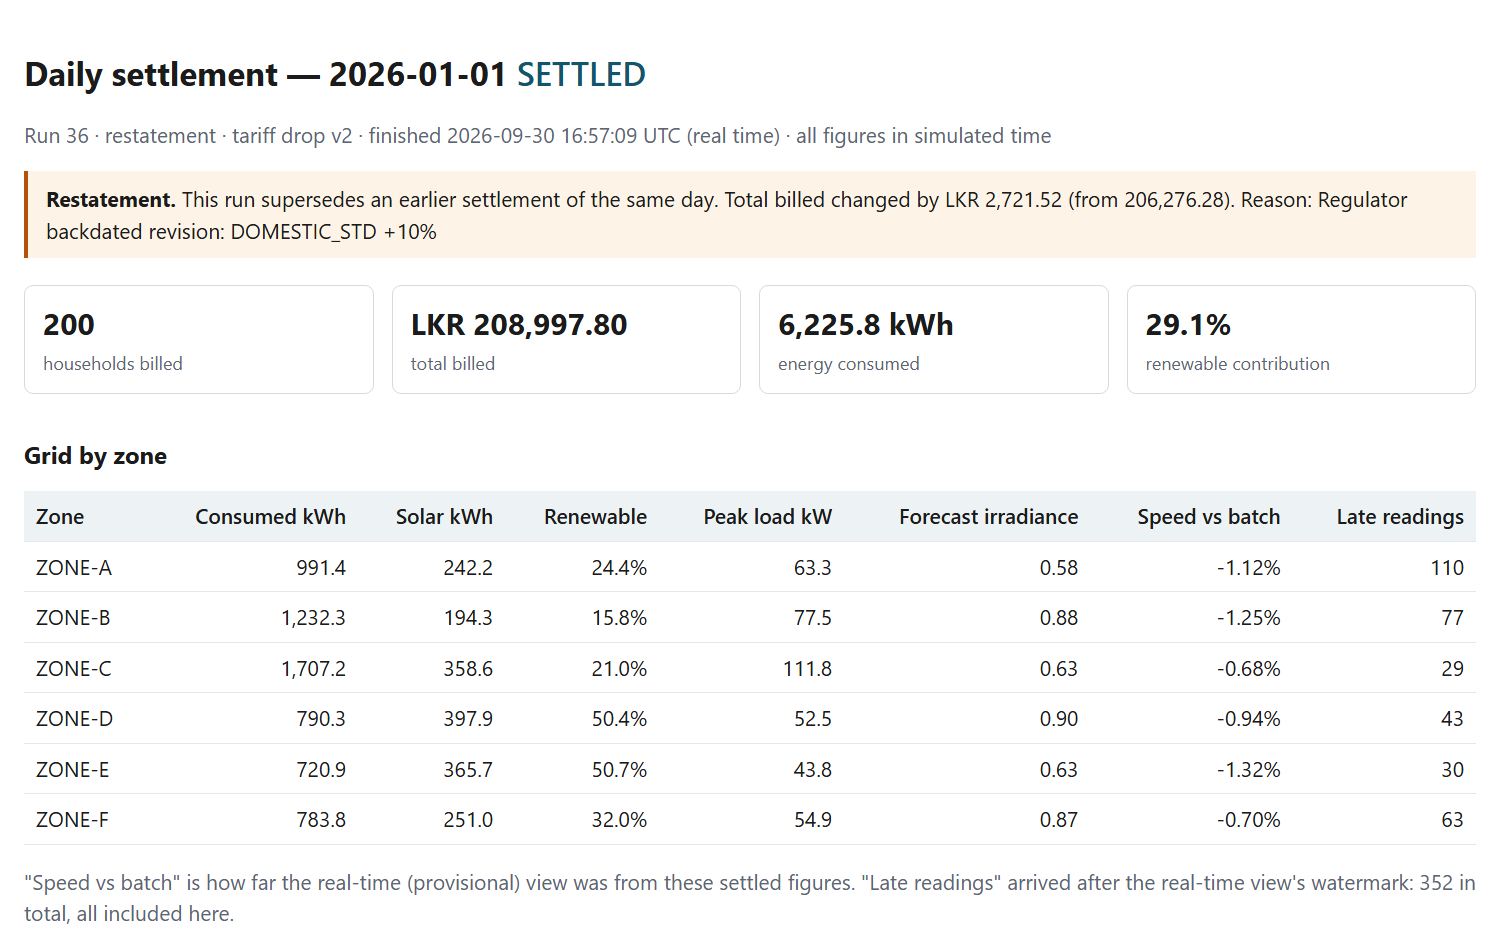
\includegraphics[width=0.84\linewidth]{figures/daily_report_restated.png}
\caption{The daily report for 2026-01-01 after a restatement (run 36, drop v2). The
highlighted note gives the change in total and its reason. ``Speed vs batch'' is the
real-time view's measured error per zone. The report continues with the largest bills
and data-quality counts.}
\label{fig:report}
\end{figure}

\begin{figure}[H]
\centering
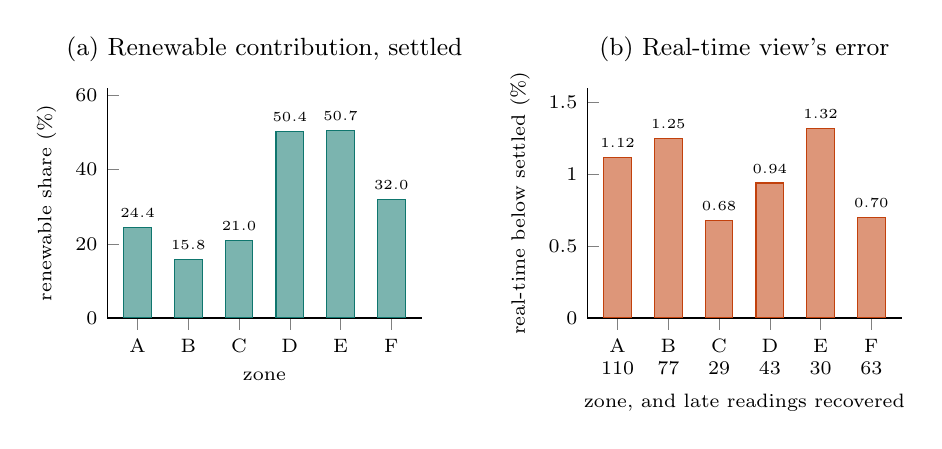
\begin{tikzpicture}
\begin{groupplot}[group style={group size=2 by 1, horizontal sep=2.1cm},
  width=0.46\linewidth, height=4.5cm, ybar, /pgf/bar width=10pt, ymin=0,
  symbolic x coords={A,B,C,D,E,F}, xtick=data, enlarge x limits=0.12,
  nodes near coords, every node near coord/.append style={font=\tiny},
  tick label style={font=\scriptsize}, label style={font=\scriptsize},
  title style={font=\small}, axis lines*=left]
\nextgroupplot[ymax=62, ylabel={renewable share (\%)}, xlabel={zone},
  nodes near coords={\pgfmathprintnumber[fixed,fixed zerofill,precision=1]{\pgfplotspointmeta}},
  title={(a) Renewable contribution, settled}]
\addplot[fill=batchc!55, draw=batchc] coordinates {(A,24.4) (B,15.8) (C,21.0) (D,50.4) (E,50.7) (F,32.0)};
\nextgroupplot[ymax=1.6, ylabel={real-time below settled (\%)},
  nodes near coords={\pgfmathprintnumber[fixed,fixed zerofill,precision=2]{\pgfplotspointmeta}},
  xticklabels={A\\110,B\\77,C\\29,D\\43,E\\30,F\\63}, xticklabel style={align=center},
  xlabel={zone, and late readings recovered},
  title={(b) Real-time view's error}]
\addplot[fill=speedc!55, draw=speedc] coordinates {(A,1.12) (B,1.25) (C,0.68) (D,0.94) (E,1.32) (F,0.70)};
\end{groupplot}
\end{tikzpicture}
\caption{Day 1, 2026-01-01. (a) Solar share of consumption by zone. (b) How far the provisional real-time
figure fell below the settled one: the speed layer under-reported every zone, by 0.7--1.3\%. The cause is
readings that arrived after its watermark, which the batch layer recovered (count under each zone).}
\label{fig:zones}
\end{figure}

\textbf{The Lambda trade-off, measured.} The speed layer was never more than 1.32\% from
the settled figure in any zone. That is ample for grid operations (\sq1). The
reconciliation counts exactly which readings the real-time view never saw: 352 that
arrived after its watermark, all recovered by settlement. Both layers apply the same
validator and the same window function, so the gap is attributable to timing, not to
diverging logic. That is precisely why billing (\sq2) must come from the batch layer.

\subsection{Restatement}
A regulator's backdated +10\% revision of the \code{DOMESTIC_STD} tariff for day 1 was
published as drop v2, and the day was restated through Airflow (\cref{tab:restate}).

\begin{table}[H]
\centering\small
\caption{Day 1 bills by tier: original settlement (run 35) against the restatement (run 36).}
\label{tab:restate}
\begin{tabular}{@{}lrrrr@{}}
\toprule
\textbf{Tier} & \textbf{Households} & \textbf{Original (LKR)} & \textbf{Restated (LKR)} & \textbf{Change} \\
\midrule
\code{DOMESTIC_HIGH} & 41 & 42{,}440.77 & 42{,}440.77 & 0.00 \\
\code{DOMESTIC_LOW}  & 51 & 1{,}420.17 & 1{,}420.17 & 0.00 \\
\code{DOMESTIC_STD}  & 86 & 21{,}884.22 & 24{,}605.74 & +2{,}721.52 \\
\code{INDUSTRIAL}    & 22 & 140{,}531.12 & 140{,}531.12 & 0.00 \\
\midrule
\textbf{Total} & 200 & 206{,}276.28 & 208{,}997.80 & +2{,}721.52 \\
\bottomrule
\end{tabular}
\end{table}

Only the revised tier changed, and the other three were identical to the cent. The
tier's energy charge rose by exactly 10.00\% (27{,}211.09 to 29{,}932.61 LKR). Its
\emph{net} bill rose by 12.4\%, because fixed charges (860.00) and solar export
credits (6{,}186.87) are unchanged while being netted against a larger energy
charge. Run 35's bills remain in the database beside run 36's.

\subsection{Performance}
\label{sec:perf}
Day 1 settled in \textbf{89\,s real time from trigger to published report}
(\cref{tab:timing}), comfortably inside the 300\,s of a simulated day. Reading many small
Parquet files dominates the cost; it is discussed in \cref{sec:limits}. The real-time view
trails the simulated clock by about 30 simulated minutes (${\approx}6$\,s real), within
the 60-second freshness target.

\begin{table}[H]
\centering\small
\caption{Settling one simulated day (28{,}245 readings in 309 Parquet files). Real seconds.}
\label{tab:timing}
\begin{tabular}{@{}lr@{\hspace{2.5em}}lr@{}}
\toprule
\textbf{Airflow task} & \textbf{s} & \textbf{Spark job step} & \textbf{s} \\
\midrule
\code{wait_for_drop}, \code{wait_for_archive} & 4 & list the archive & 9.1 \\
\code{quality_gate} & 2 & read and re-validate & 24.9 \\
\code{settle} (incl.\ 24\,s start-up)$^{*}$ & 74 & deduplicate & 2.9 \\
\code{reconcile} & 2 & aggregate & 9.7 \\
\code{report} & 3 & write snapshot & 2.8 \\
 & & bill and commit & 0.1 \\
\midrule
\textbf{Trigger to report} & \textbf{89} & \textbf{Spark total} & \textbf{49.5} \\
\bottomrule
\multicolumn{4}{@{}l}{\footnotesize $^{*}$Starting the child process, the JVM and Python, and the job's own re-check of the drop.}
\end{tabular}
\end{table}

\subsection{The business dashboard}
A Streamlit dashboard answers the business question for a non-technical reader. It reads
\emph{only} the serving API, so it cannot disagree with the merge rule. Its five pages
cover the current grid, zone history across days, one settled day, household bills with
their restatement history, and every settlement run. Two design rules make the
provisional/settled distinction impossible to miss:
\begin{enumerate*}[label=(\roman*)]
  \item source is shown by colour \emph{and} words, blue for \textsc{settled} and orange
  for \textsc{provisional}. That pair was validated as colour-blind safe (worst CVD
  $\Delta E$ 24.7 in light mode, 26.8 in dark, against a target of 8), and each source
  keeps its colour when the other is absent;
  \item load and solar share are always separate charts, never one chart with two
  y-axes.
\end{enumerate*}
Every chart has a table view.

\begin{figure}[H]
\centering
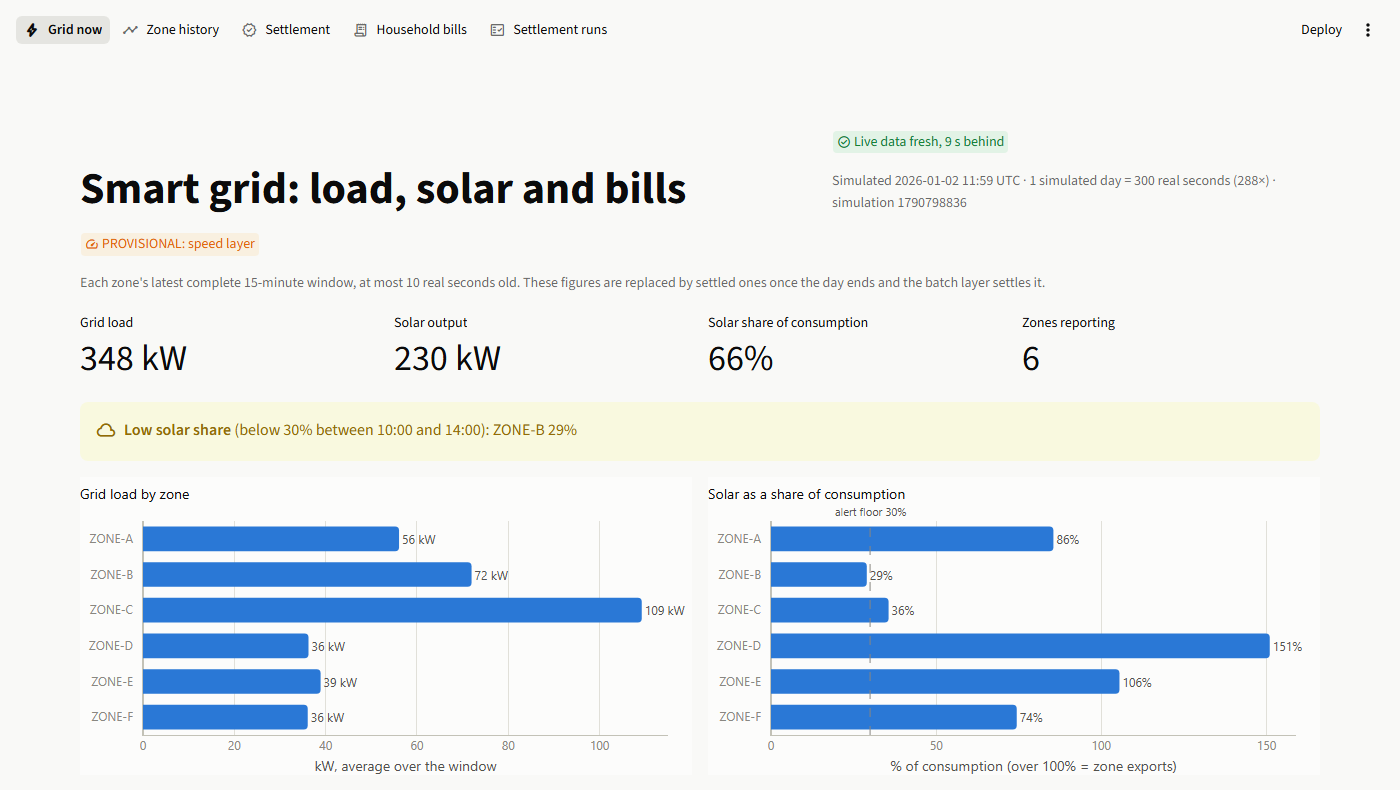
\includegraphics[width=0.93\linewidth]{figures/dashboard_grid_now.png}
\caption{Grid now, at simulated 2026-01-02 11:59, during the live run. Each zone's
latest complete window, 9\,s old in real time and labelled \textsc{provisional}. ZONE-B
triggered the low-solar warning at 29\% against a 30\% floor, which applies only
between 10:00 and 14:00: at night every zone is at 0\%, which is not news. The floor was
calibrated on the simulation, where midday zone shares run from 25\% to 180\%.}
\label{fig:dash-grid}
\end{figure}

\begin{figure}[H]
\centering
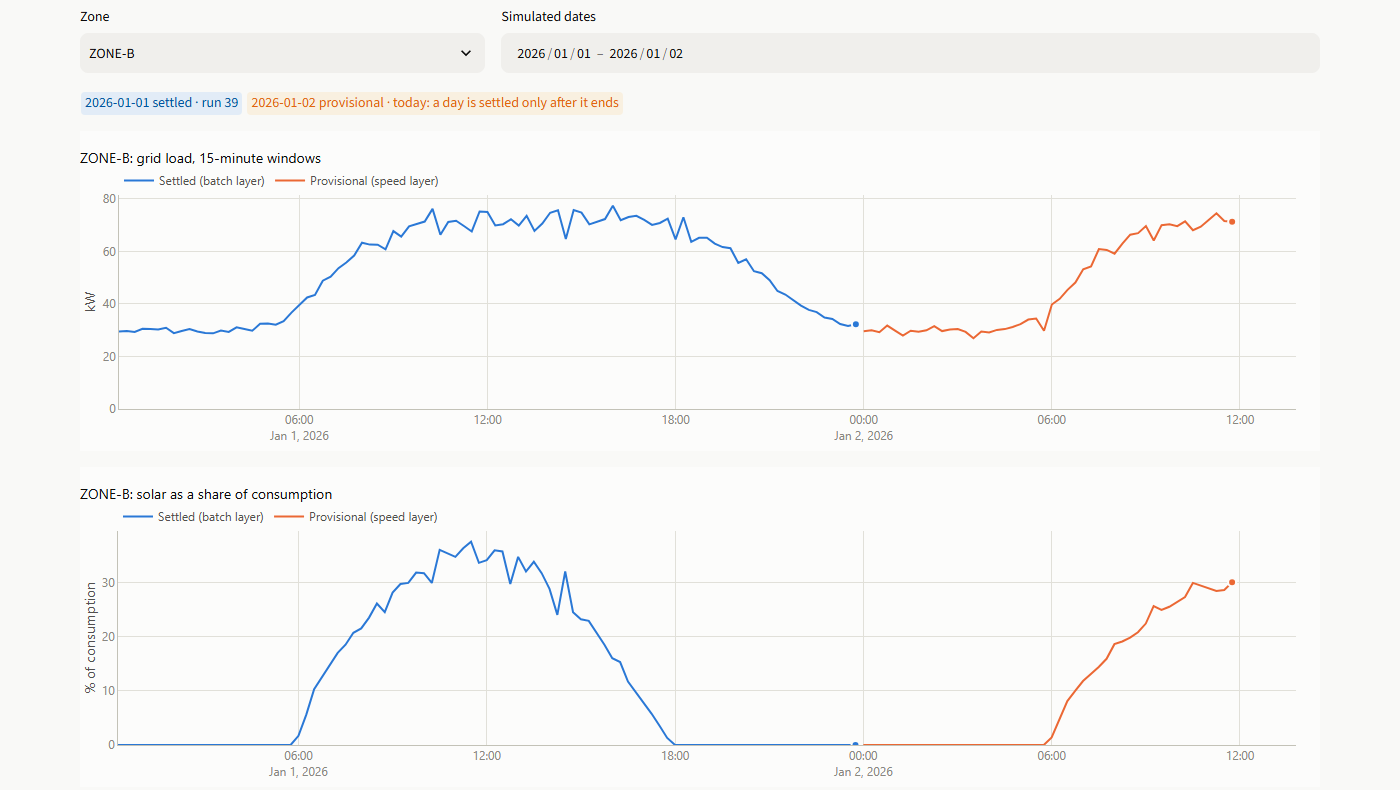
\includegraphics[width=0.93\linewidth]{figures/dashboard_zone_history.png}
\caption{Zone history: the merge rule on one chart. Day 1 is settled (run 39, blue),
recomputed by the batch layer with its late readings. Day 2 is today, provisional from
the speed layer (orange). The day badges above the charts say which layer served each day.}
\label{fig:dash-history}
\end{figure}

The household page makes restatement visible to a billing clerk. In the same run, a
backdated +10\% \code{DOMESTIC_STD} revision was restated through Airflow. For household
HH-00071 the page then listed both settlements of day~1: 825.67\,LKR under drop v1
(run 39), and 907.24\,LKR under drop v2 (run 40), marked as the bill now shown, with the
regulator's reason.

\pending{Section 10. Add the Grafana operations dashboard (one screenshot, two or three
sentences) and an Airflow grid-view screenshot showing scheduled, restated and
gate-refused runs.}

% ============================================================================
\section{Limitations, trade-offs and production scale}
\label{sec:limits}
% ============================================================================

\textbf{Deliberate simplifications of the demo.}
\begin{itemize}
  \item \textbf{Single Kafka broker, replication factor 1.} No fault tolerance. Production would use three brokers, replication 3 and \code{min.insync.replicas=2}.
  \item \textbf{Spark in local mode} (\code{local[4]}) in one container per layer, rather than a cluster.
  \item \textbf{Airflow standalone} with LocalExecutor, a UI without login, and its metadata in the serving PostgreSQL instance. Acceptable locally, never shared.
  \item \textbf{Tariff blocks are pro-rated to one day.} A real utility accumulates month-to-date consumption and charges the marginal block.
  \item \textbf{Compressed time exaggerates throughput}: 288 simulated days pass in one real day, so our throughput figures are not production figures.
  \item \textbf{Security}: development credentials in \code{.env}, no TLS. MinIO runs from a pinned archive image, because MinIO withdrew its public images, and it receives no security updates.
\end{itemize}

\textbf{Trade-offs we accepted, with their measured cost.}
\begin{itemize}
  \item \textbf{Two processing paths} remain Lambda's real cost: two deployments (a
  streaming container and the Airflow image) must pin the same Spark version. We hit
  exactly this when Airflow's constraints pinned a different PySpark.
  \item \textbf{Python validation inside Spark}, rather than native expressions, buys one
  provably shared rule set at a throughput cost. Reading and re-validating a day is
  the largest step in settlement (24.9\,s).
  \item \textbf{Small files.} The speed layer writes a file per zone per micro-batch: 309
  files for one simulated day. Settlement reads them rather than rewriting the raw
  partition, because late readings can still arrive after a day is settled. Without
  a table format, rewriting that partition could delete a file written during the
  rewrite. Each run instead writes one compacted snapshot of what it settled.
  \item \textbf{The watermark} trades completeness for freshness. At 30 simulated minutes
  the real-time view is within 1.3\% of settled. A longer watermark would narrow the
  gap and delay the view.
  \item \textbf{Resources.} The full stack needs about 6\,GB of memory while settling.
  On a starved host, settlement slowed from 90\,s to over 7 minutes, and the Docker
  runtime once failed. The README states this requirement.
\end{itemize}

\textbf{What we would do differently at production scale.}
\begin{enumerate}
  \item \textbf{A table format (Apache Iceberg or Delta Lake) over the master dataset and landing
  zone.} Restatement and compaction become transactional; time travel replaces our
  version folders and manifests with the same semantics; and small files are compacted
  in place.
  \item \textbf{Compile the \code{FieldSpec} rules to native Spark expressions}, keeping one
  declaration but removing the Python round trip.
  \item \textbf{A schema registry} with Avro or Protobuf instead of JSON, so schema changes are
  checked at the producer rather than discovered in the dead-letter topic.
  \item \textbf{Re-evaluate Flink with an Iceberg sink.} If a stream processor can recompute
  targeted historical partitions cheaply, the batch layer's reason to exist weakens and
  Kappa becomes viable. This is the condition under which we would revisit this decision.
  \item \textbf{Cluster deployment}: Spark on Kubernetes, Airflow with a Kubernetes executor
  and its own database, and managed object storage.
\end{enumerate}

% ============================================================================
\section{Individual contributions}
\label{sec:contrib}
% ============================================================================

The project was planned and reviewed jointly. Design decisions were agreed in group
discussion and recorded as ADRs, and each member reviewed the others' code before it
was merged. Primary responsibilities were divided as follows.

\begin{table}[H]
\centering\small
\caption{Division of work.}
\label{tab:contrib}
\begin{tabularx}{\linewidth}{@{}>{\raggedright\arraybackslash}p{1.6cm}>{\raggedright\arraybackslash}X>{\centering\arraybackslash}p{1.35cm}@{}}
\toprule
\textbf{Member} & \textbf{Primary responsibilities} & \textbf{Share} \\
\midrule
Ravindu & Overall architecture and the Lambda-versus-Kappa decision; lead author of the ADRs.
Infrastructure: the Docker Compose stack (Kafka, PostgreSQL, MinIO) and the Spark image.
The shared foundation: simulated clock, configuration, shared validation module and its
parity tests. The speed layer (Spark Structured Streaming). End-to-end integration and
verification runs; report editing. & 36\% \\
\addlinespace
Amami & The streaming source: smart-meter simulator, energy and solar model, fault
injection. The billing model: tariff schedule, block tariffs, exact decimal arithmetic,
subsidy and export credit. Observability: Prometheus metrics, Grafana dashboards and
alert rules. The Streamlit business dashboard. Report sections on data sources,
observability and results. & 32\% \\
\addlinespace
Oshani & The daily batch source: versioned drops, manifests and the quality gate. The batch
layer: the Spark settlement job, Airflow DAGs, reconciliation, daily report and
restatement. The serving API and its merge rule. Report sections on the batch and
serving layers, and limitations. & 32\% \\
\bottomrule
\end{tabularx}
\end{table}

\begin{thebibliography}{9}
\small
\setlength{\itemsep}{1pt}
\bibitem{marz2015} N.~Marz and J.~Warren, \emph{Big Data: Principles and Best Practices of Scalable Realtime Data Systems}. Manning, 2015.
\bibitem{kreps2014} J.~Kreps, ``Questioning the Lambda Architecture,'' O'Reilly Radar, July 2014.
\bibitem{kleppmann2017} M.~Kleppmann, \emph{Designing Data-Intensive Applications}. O'Reilly, 2017.
\bibitem{spark} Apache Software Foundation, \emph{Structured Streaming Programming Guide}, Apache Spark 3.5 documentation.
\bibitem{airflow} Apache Software Foundation, \emph{Apache Airflow 3.1 documentation}.
\bibitem{kafka} Apache Software Foundation, \emph{Apache Kafka documentation}, including KRaft mode.
\end{thebibliography}

\end{document}
